%----------------------------------------------------------------------------------------
%	Project management
%----------------------------------------------------------------------------------------
\chapter{Project management} % Main chapter title
\label{Chapter5} % For referencing the chapter elsewhere, use \ref{Chapter5}

This section covers the management of the project, including the project's lifecycle during development, the software testing involved with ensuring all operations are functional, and what methods were used to mitigate risk guaranteeing the project's success.

%----------------------------------------------------------------------------------------
%	1. Project life cycle
%----------------------------------------------------------------------------------------

\section{Project life cycle}

Development of the project utilised the agile approach consisting of two-week sprints focused on delivering features. Rather than building and implementing each layer, the system was built using vertical slices. Each requirement consisted of a slice of the project from UI to API to the database and back again. Each slice was added over time to assemble the complete system which follows the FDD approach.

The full list of completed actions for each week during the planning stage and each sprint during the development stage has been tracked in Trello (Appendix \ref{AppendixA:Trello}), and time management in the Gantt chart (Appendix \ref{AppendixA:Gantt}).


\subsection{Environment setup}
Development started with setting up the development environment, which included creating the GitHub repository and linking it to the development system.

The Trello board was then created to list all system requirements and allow for tracking work completed each sprint.


\subsection{MVP - Login and Members}
A minimum viable product (MVP) was created to start the development of the system stack. The minimum the business requires to start is a member storage and view combined with a method of access control through a login system.

\begin{figure}[ht!]
    \centerline{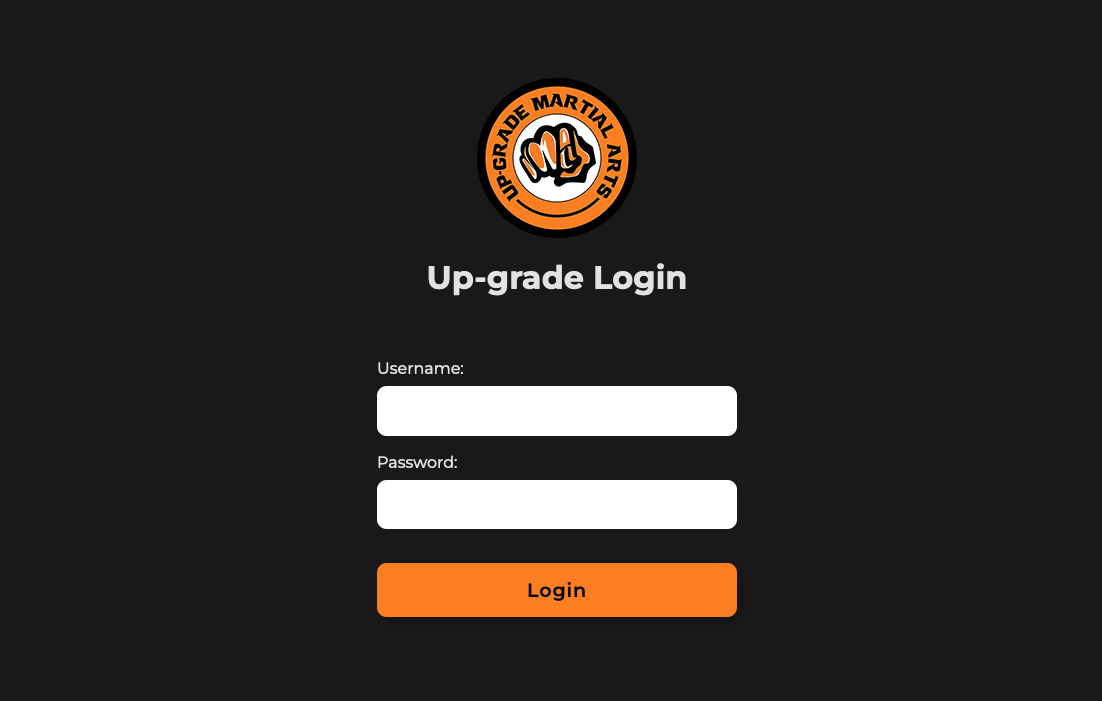
\includegraphics[width=.9\linewidth]{login.png}}
    \caption{Implemented login screen including logo and form}
    \label{fig:login}
\end{figure}


The login system \parencite{adams_basic_2018} \parencite{macharia_session_2021} is vital in securing the system from unauthorised access to stored personal and business data. Access control became the first system implemented for this reason.

The database was initially created with the 'users' table to store the staff usernames and passwords. The creation of this table was added to the schema file, and default login details were provided in the seed file.

The API was then initialised to support a POST endpoint to receive login data and provide a response if a matching record was found in the database. The 'express' package provided the interface for receiving HTTP requests, and the 'pg' package for interfacing with the database. The database connection details were added through environment variables since they change and connection made using a connection component.

\begin{figure}[ht!]
    \centerline{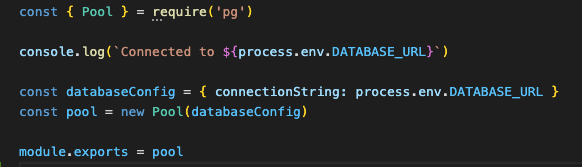
\includegraphics[width=.9\linewidth]{dbconn.png}}
    \caption{Database connection component using environment variables to connect}
    \label{fig:dbconnect}
\end{figure}

Research into best practices \parencite{page_how_2023} revealed the need to store passwords as encrypted strings \parencite{gauravaram_security_2012} rather than plain text. This encryption is to prevent system administrators from gaining customers' login data, which they could exploit, and also stop malicious actors such as hackers from using the details should the database become compromised or leaked.

\begin{figure}[ht!]
    \centerline{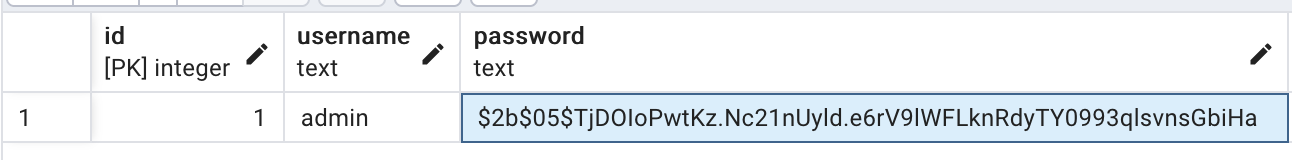
\includegraphics[width=.9\linewidth]{encrypted-password.png}}
    \caption{Salted and hash encrypted password}
    \label{fig:password}
\end{figure}

The 'bcrypt' package was added to provide functionality for salting and hashing the received passwords. Now, passwords stored in the database are encrypted (Figure~\ref{fig:password}). The received password is put through the same method to salt and hash, then compared to check if login details match.

If successful, the API returns a JSON Web Token (JWT) containing necessary user data, such as their ID, alongside an expiration date and time when the token is no longer usable. This token can only be opened by the server making the data stored inside secure and preventing impersonation from maliciously crafted tokens.

This token can now be appended to data requests where the server can open and verify credentials allowing a request to succeed. This verification method within the API was created as middleware which can be attached to any endpoint, enforcing the requirement of a valid bearer token to access the data.

A new form was created in the UI, which allows entering a username and password in combination with a button to submit the login request. This request is sent to the API and handles the response received. If the token is returned with a 200 response code, the token is stored, and the app component is rendered through React's hooks. A corresponding error message is shown to the user if an error response is received.

With the app secured with access control, data can now be stored. A new table was created to hold member data based on the normalised form created during development. This table was added to the schema file for generation upon new database creation.

\begin{figure}[ht!]
    \centerline{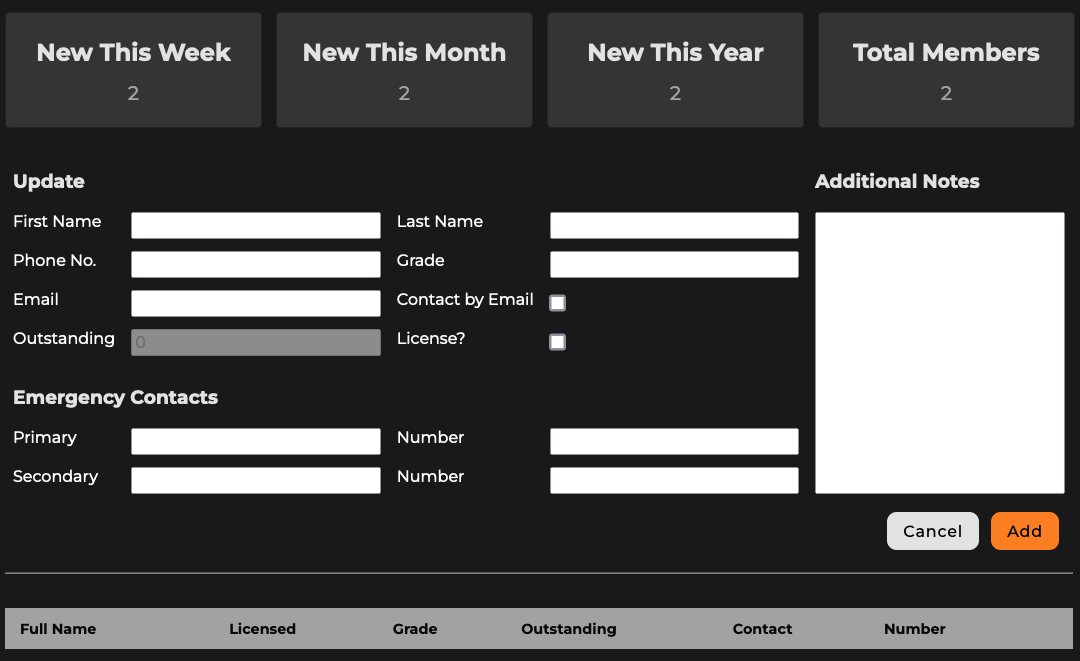
\includegraphics[width=.9\linewidth]{members-page.png}}
    \caption{Implemented members page}
    \label{fig:members-page}
\end{figure}

Three endpoints were added to the API to support viewing all members, adding a new member and editing an existing member referenced by ID. In addition, validation of inputted data and verification of a bearer token was added as middleware, preventing error cases such as missing required fields and expired or missing tokens.

Finally, the UI must support viewing all member data, the input of new members who are registering and updating existing members already recorded in the system.

A table view was first created to display all members. A fetch request to the API returns an array of members, which are mapped for easy searching based on their ID. This map is then iterated over to create the rows in the table.

Afterwards, a form was created to input new member data, which could then be submitted to the API for storage. The form had the required fields match those found in the database and would be verified within the API middleware. This consistency would prevent accidental errors in input by preventing submission without the requirements met.

This form could be reused to update existing members if provided with an ID. The table was altered to support an 'onClick()' event where a function could be performed when the selected row was clicked. This function sets an active id variable rendering the form with the data filled into the fields for altering. The active id also changes the behaviour of the form submission by changing the request from a POST to a PATCH utilising the update route instead of the add route (Figure~\ref{fig:members-patch-post}).

\begin{figure}[ht!]
    \centerline{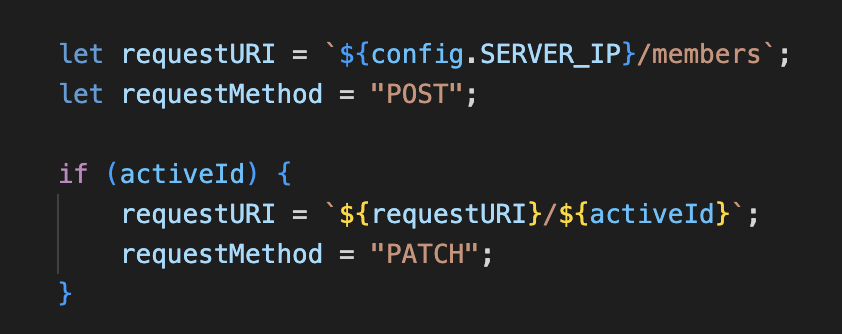
\includegraphics[width=.6\linewidth]{post-or-patch.png}}
    \caption{If check for adding or updating a member's record}
    \label{fig:members-patch-post}
\end{figure}


\subsection{Sprint 1 - Lessons}

This first sprint focused on storing lessons and the required lesson types. In order for lessons to be stored, their lesson types must be stored first which they can then reference. The lesson types consists of "Boxing (Kids)", "Boxing (Adults)", "Kickboxing (Kids)", "Kickboxing (Adults)" and "Yoga".

A table was created to hold these values along with a referencable ID (Figure~\ref{fig:lesson-types-schema-sql}). The lesson types are added as non-editable, static values to the database (Figure~\ref{fig:lesson-types-seed-sql}). A route was added to get all rows. Since the values are static, there is no need for POST or PATCH to handle adding or updating respectively.

\begin{figure}[ht!]
    \centerline{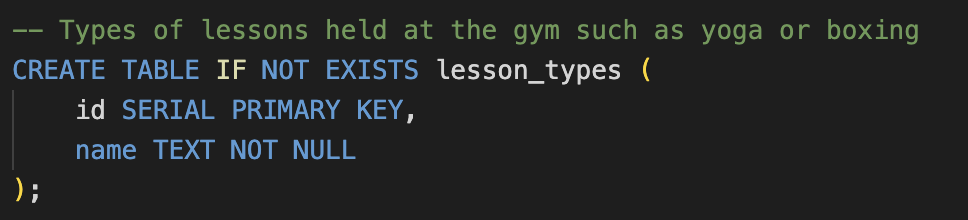
\includegraphics[width=.9\linewidth]{lesson-types-sql.png}}
    \caption{Lesson types sql schema}
    \label{fig:lesson-types-schema-sql}
\end{figure}

\begin{figure}[ht!]
    \centerline{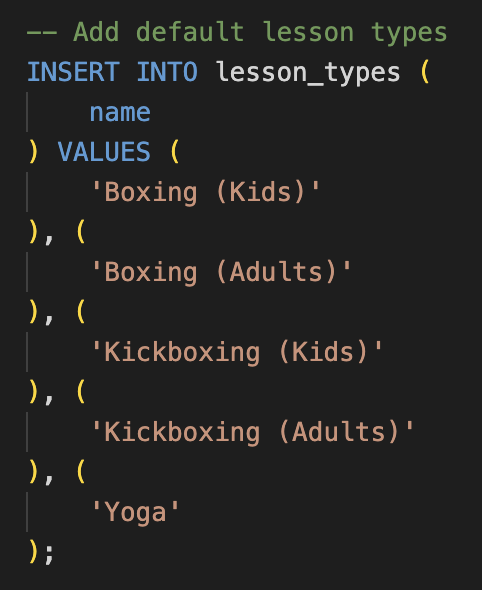
\includegraphics[width=.4\linewidth]{lesson-types-seed-sql.png}}
    \caption{Lesson types sql seed}
    \label{fig:lesson-types-seed-sql}
\end{figure}

The interface also matches this static state of the table by not providing a method to edit the data. The records are instead stored within the user interface as a map which is retrieved upon login. This way we prevent future requests and unnecessary network requests for the data by keeping a single local copy.

Lessons can be added now that the types have been defined and are retrievable. The lesson were created by first creating the database schema. The table contains a foreign key linked to the lesson types table. Now the lessons can contain a referenced type. This is useful for searching functionality and in the future for lesson attendance based on lesson type.

\begin{figure}[ht!]
    \centerline{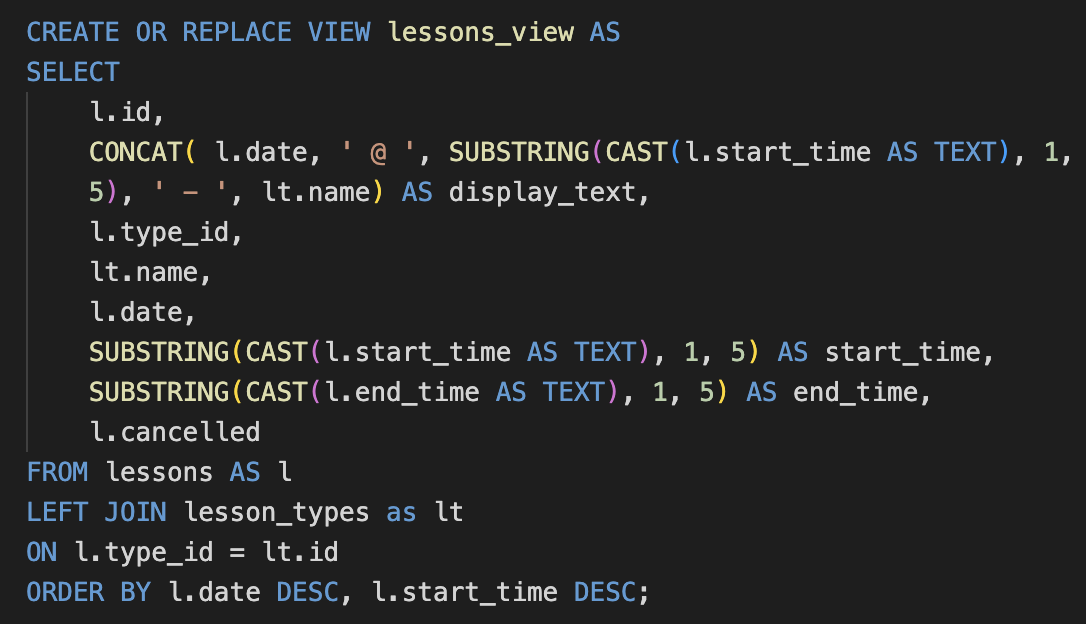
\includegraphics[width=.8\linewidth]{lessons-view-sql.png}}
    \caption{Lesson view sql schema}
    \label{fig:lesson-view-schema-sql}
\end{figure}

A view was also created within the database to get the data including labels from the linked table as text (Figure~\ref{fig:lesson-view-schema-sql}). This prevents the need to manually search each table and instead get all necessary values in a single query. This also results in lower network utilisation through less queries.

Next the routes were added to the API for requesting all lessons, adding new lessons and updating existing lessons. This followed the same structure as the customers table. The get request references the view providing this useful reduced search information.

Finally adding new page to the UI to interact with the API endpoints created for input, view and updates. New form elements had to be utilised, including date and time selectors.

\begin{figure}[ht!]
    \centerline{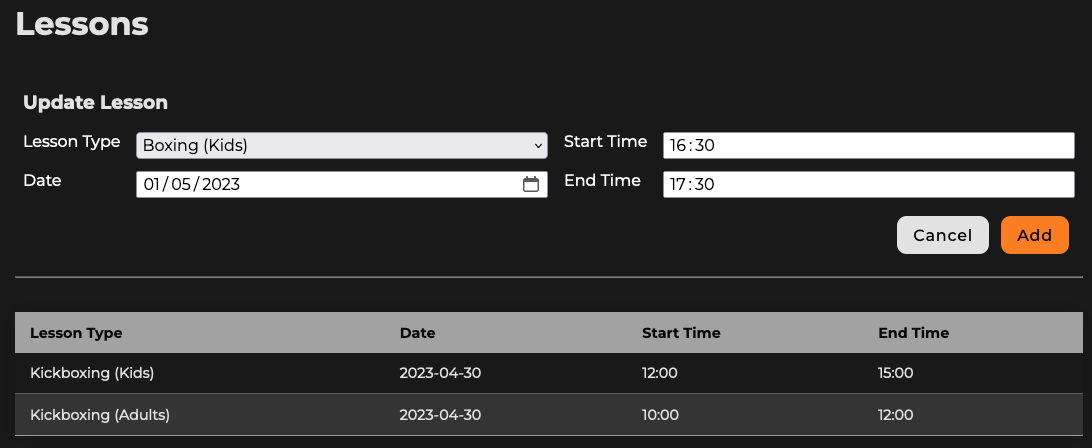
\includegraphics[width=\linewidth]{lessons-page.png}}
    \caption{Implemented lessons page with form and table}
    \label{fig:lessons-page}
\end{figure}

A more complex element was the drop-down menu. Lessons have required lesson types. The selected value is that of the ID rather than the text contained within. This was complex and required creating a new customisable component which can now take any map of values and create a drop-down. When the value is changed, a callback function can update a stored variable and trigger other changes too.

\begin{figure}[ht!]
    \centerline{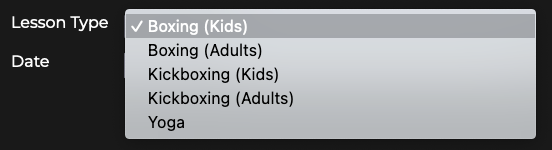
\includegraphics[width=\linewidth]{custom-drop-down.png}}
    \caption{Custom drop-down menu using data fetched from the API}
    \label{fig:drop-down}
\end{figure}

This sprint's work lays the foundation for pricing, purchasing and eventually attendance of members to these lessons.


\subsection{Sprint 2 - Lesson Pricing}
The pricing structure requires different prices for different lesson types and durations. We have the lesson types defined from the last sprint so the lesson purchase types to differentiate the prices is now required.

The table was created to store the purchase types: day single, weekly single, weekly double, weekly triple, and weekly unlimited. This was added to the schema file and the database updated to include the new table.

Using these two tables, the table lesson pricing was created and prices added to the seed file. This table combines the lesson types and purchase types to allow the storage of the comprehensive price list.

\begin{figure}[ht!]
    \centerline{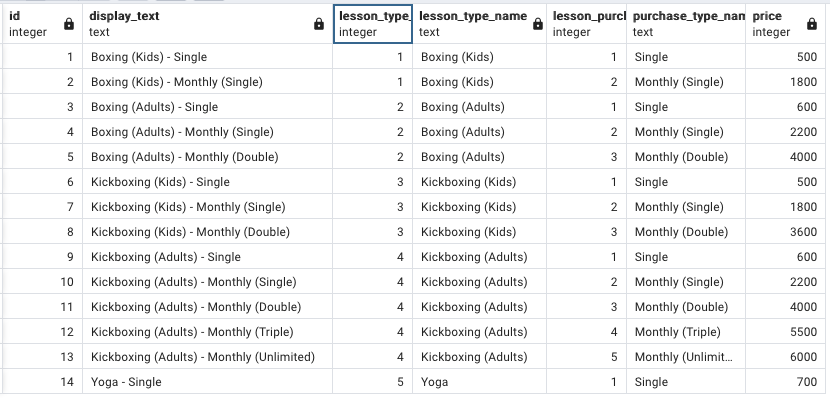
\includegraphics[width=\linewidth]{lesson-pricing-tables.png}}
    \caption{Database view of lesson pricing table with left joined lesson type and purchase type}
    \label{fig:lesson-price-view}
\end{figure}

Routes were added to the API allowing requests for the purchase types and the prices. The prices are retrieved from a view which includes the lesson and purchase types. This aids in the display of these prices in drop-down selection boxes.

During planning these were listed as static values, however prices may require updating in the future requiring a patch to the database to do this. This was a large oversight during the design stage. Although there is no interface designed, a route for updating the prices has been included for easier developer maintenance.

\begin{figure}[ht!]
    \centerline{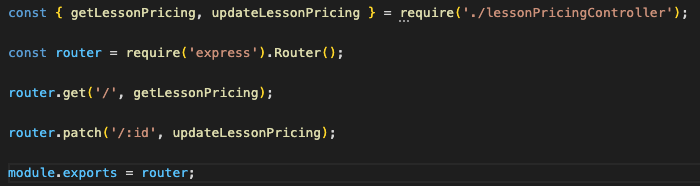
\includegraphics[width=\linewidth]{pricing-patch.png}}
    \caption{Update route for lesson pricing}
    \label{fig:pricing-patch-router}
\end{figure}

The purchase types and prices were added to the interface for storage on login. With these values now stored, lesson purchasing and payments can be focused on next. This will lead gracefully onto tracking the attendance in a later sprint.


\subsection{Sprint 3 - Lesson Purchasing}
With lessons and pricing now functional, a record of payment and methods are required to start making lesson purchases.

Payment methods are a simple static table which holds the different payment methods the business supports. They have explicitly specified they only accept cash and card payments only. The data could be stored statically within the application and text saved however for indexing and data consistency, a new table for payment methods was created.

Payments were then created to hold a record of all income made from lessons. The payments consist of the member who made the payment, method of payment, the total amount paid and when the payment was made.

If the prices can now update in the future, we cannot rely on the stored prices to track history purchases and payments. For this reason, the tables include their own prices which reflect the calculated price at the time of purchase.

\begin{figure}[ht!]
    \centerline{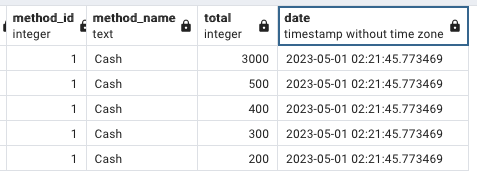
\includegraphics[width=.8\linewidth]{payments-table-snapshot.png}}
    \caption{Database payments table tracks total without links}
    \label{fig:payments-total}
\end{figure}

Lesson purchases combine the member, lesson type, duration through purchase type and the payment made to track what members have made what purchases. This increases the accuracy of the data stored which can be further used for business analytics.

Static route was added for payment methods and like all prior static data is retrieved upon login. The payments are handled internally within the API as a middleware. The lesson purchase API route includes this payment middleware by using the submitted data to determine the payment data and adds it when a lesson is purchased. This automated nature and removal from the UI simplifies the external interface removing unnecessary endpoints and making interaction far easier.

Lesson purchases screen created using the wireframe and interfaces with the API endpoint. A price list is shown on this screen which required uses the prices data the interface holds. This is useful when customers inquire about prices removing the need for print outs or searching files on the computer or phone.

% Add screenshot of price list table and purchase form

The attendance could be tracked using this, however would require a great deal of calculation upon each validation request. To increase efficiency and improve the scalability of the system, the token system will be implemented in the next sprint.


\subsection{Sprint 4 - Tokens}
Members can now purchase lessons and now must be able to use these purchases to attend lessons.

In need of an efficient system to track attendance based on week and month, a ticket system was implemented to solve this issue. Based on lesson purchase type and lesson type, a token representing a valid pass for a particular lesson during a particular period would solve the problem.

Also solved the issue of a free first lesson for new members. A token without a set lesson type could be used to be a general pass, and an expiration date of 1 year would be sufficient, which the member could claim.

First a table to track the tokens issued. The token is issued to a member with an activation start date for when the token starts being valid and an expiration date when the token is no longer usable. Finally, there is a used flag which can be set to invalidate the token however keep it in the system for metrics data.

A view was created of these tokens to only show unused tokens making further searches faster by working on a subset of the data.

\begin{figure}[ht!]
    \centerline{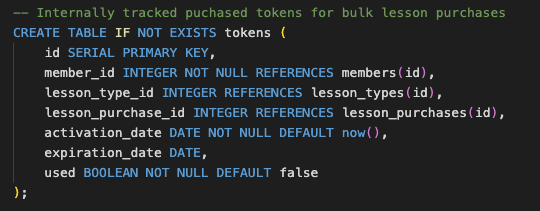
\includegraphics[width=.8\linewidth]{token-table.png}}
    \caption{Token table schema}
    \label{fig:token-table}
\end{figure}

An endpoint to request the next valid token based on the member id was created for the future attendance screen. This was done by first querying for tickets that are for the active lesson type. On the subset of results they are checked if they are not yet used, the start date is before the current date and the expiration is after the current date. If a valid token is available, the ID may be used to allow attendance to a lesson. This was tested with custom crafted tokens.

To generate tokens is more complicated than filtering. First the API requires a member, lesson type and purchase type to determine who gets the tokens, how many to generate and what date range each are for. The purchase type table was modified to include the number of tokens to generate, the duration in days each token is valid for and how many weeks of these tokens to create. The lesson purchase route was extended to include the generate tokens middleware. Now when lessons are purchased, tokens which correlate to the purchase are generated and stored for the specified member. 

\begin{figure}[ht!]
    \centerline{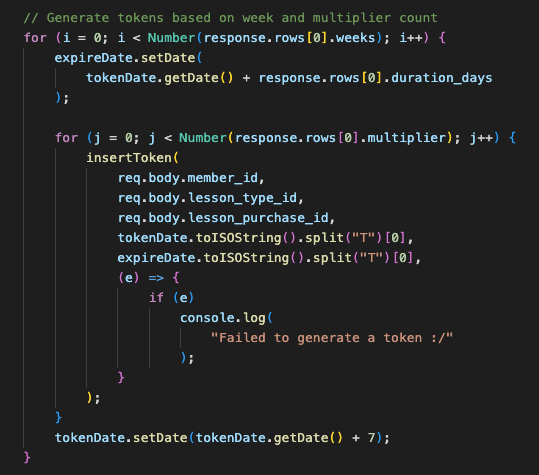
\includegraphics[width=.8\linewidth]{generate-tokens.png}}
    \caption{Code to generate tokens on lesson purchase}
    \label{fig:purchase-gen-tokens}
\end{figure}

These tokens can now be used to attend lessons which is the focus of the next sprint, sprint 5.

\subsection{Sprint 5 - Attendance}
The next step is to track member attendances to lessons. The attendance is made up of members in combination with lessons. The limiting factor which has now been addressed is the tokens allowing participation in particular lessons. The attendance date is tracked for metrics and statistics which can be displayed on the dashboard.

In the intial iteration of the attendance tracking tokens were not required and the attendance was tracked by the member and lesson type. This was later changed to require tokens to attend once attendance was implemented.

\begin{figure}[ht!]
    \centerline{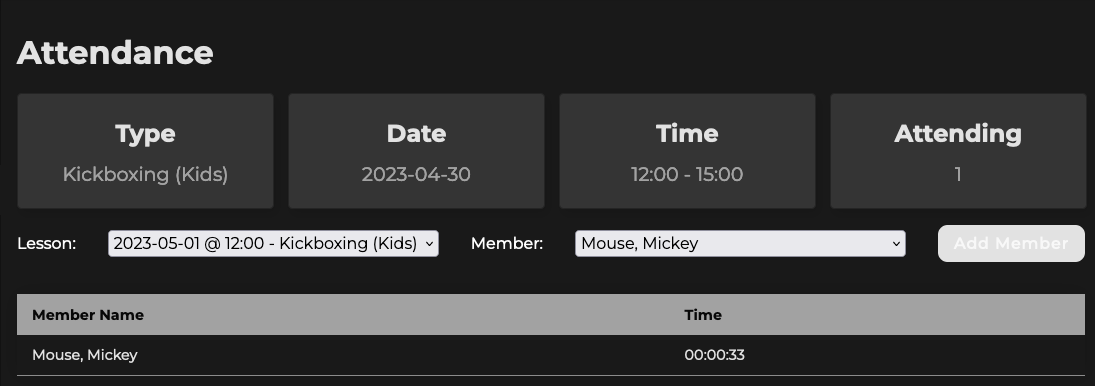
\includegraphics[width=\linewidth]{attendance-screen.png}}
    \caption{Attendance implemented screen}
    \label{fig:attendance-screen}
\end{figure}

The next hurdle lies with members wishing to pay later and within the same screen. An option for members to pay now or later was added as a component that can trigger the same purchase endpoint; the lesson purchase screen has already implemented the required behaviour making extension of this simple in thanks to the MVC architecture.

To manage pay later, attendances could be made without a token. This would prompt the API to append the price of the lesson to the outstanding amount in the member's record.


\subsection{Sprint 6 - Statistics and Metrics}
With the core functionality the receptionist will be utilising during everyday operations, the metrics and statistics will be helpful for managers' needs adding through a dashboard immediately visible upon login.

\begin{figure}[ht!]
    \centerline{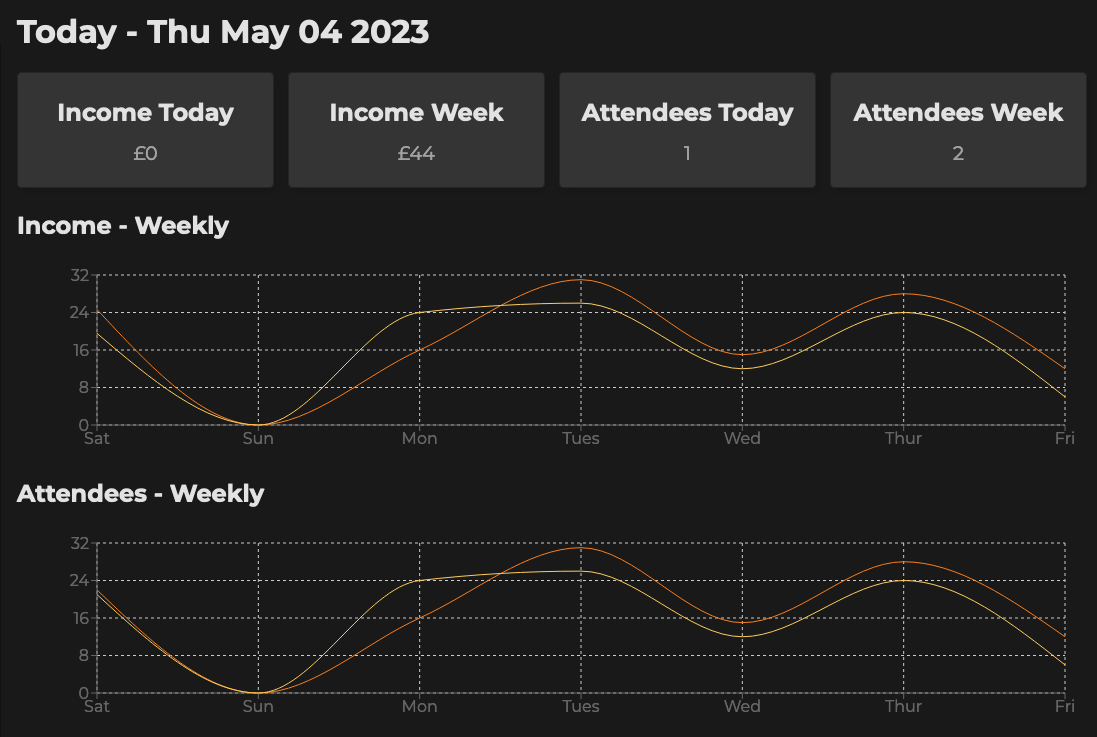
\includegraphics[width=.8\linewidth]{dashboard.png}}
    \caption{Dashboard implemented screen}
    \label{fig:dashboard-screen}
\end{figure}

For a more visual reprenstation of the data, two graphs were used to show the weekly income and attendances. Since these will closely correlate with each other, it will be clear to see the trends of both and compare them at a glance. To create these graphs the data must be retrieved from the database and formatted into a JSON object which can be used by the graphing library. The graphing library used was Chart.js which is a free open source library for creating graphs and charts. The library was chosen for its simplicity and ease of use. The data is displayed on the dashboard screen below the cards.


\subsection{Sprint 7 - Final Deployment}
For the final deployment, a domain name was aquired to provide a single point to access the web application. The domain name was purchased from name.com and the hosting was provided by Linode. The domain name was linked to the hosting by adding A records pointing to the Linode server host. The hosting was configured to run the web application using a virtual private server (VPS) running Ubuntu 20.04. The web application was deployed to the VPS using Git and the web server was configured to serve the application.

\begin{figure}[ht!]
    \centerline{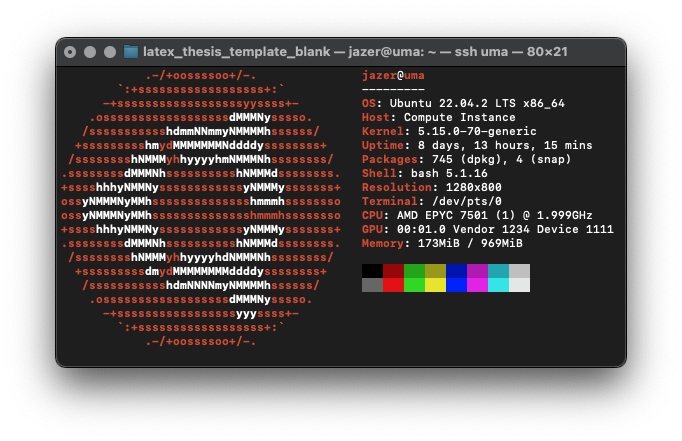
\includegraphics[width=\linewidth]{server.png}}
    \caption{Server hosting the web application}
    \label{fig:server}
\end{figure}

The web server used was Nginx which is a free open source web server. The web server was configured to use a firewall to block all traffic except for the required ports. The web server was also configured to use a secure sockets layer (SSL) certificate to encrypt the traffic between the web server and the client.

The SSL certificate was provided by Let's Encrypt which is a free open source certificate authority. The SSL certificate was configured to automatically renew every 90 days. The web server was configured to redirect all HTTP traffic to HTTPS to ensure all traffic is encrypted.

\begin{figure}[ht!]
    \centerline{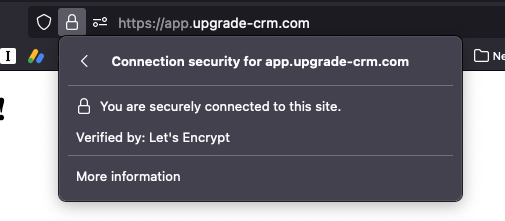
\includegraphics[width=.8\linewidth]{ssl.png}}
    \caption{Website secured with Let's Encrypt SSL certificate}
    \label{fig:ssl}
\end{figure}

\subsection{Sprint 8 - Bug Fixing and Report}
The final sprint was focused on bug fixing and writing the report. The bug fixes were focused on the issues that were found during the testing phase. These were quite few and far between thanks to regular unit tests on the developed components. The larger end-to-end tests results showed some inconsistencies when these components interacted together. This was valuable as the end-to-end operations are what the end user will be experiencing when interacting with the system. 

The report was written in LaTeX and was focused on the design and implementation of the web application from start to finish. Great care was taken to include all the details of the development process and the reasoning behind the decisions made. The report was also written in a way that it could be used as a guide for future developers to understand the system and how it was developed making futher development easier and more efficient.


%----------------------------------------------------------------------------------------
%	2. Software testing
%----------------------------------------------------------------------------------------

\section{Software testing}

Testing is vital to the development to ensure a high-quality user experience and prevent bugs and other inconsistencies from occurring within the system.

\subsection{Testing methods}
Testing can be approached from a black-box or white-box technique. Black-box testing is where only the inputs and outputs are of concern, with the internal structure unknown. In contrast, white-box testing reveals the inner workings of an operation, and further testing to interact with the internals is the focus.

Black-box testing is beneficial in the end-to-end validation of a function, operation or even user stories since it can provide a similar interaction that the end user will experience. Unfortunately, this testing is most commonly performed manually; each test is carried out by either the developer or a manual tester.

White-box testing focuses more on the functionality of smaller components within the system, such as algorithms and specific functions. Since the code is visible and followed, developers can use automated tests to guarantee that functions behave as expected.

In both methods, different parameters yield different functionality and responses from the application. These can exist as sunny-day scenarios where all inputs are what is expected, edge cases where the limits of inputs are tested but are still within bounds and finally, error scenarios where the input falls outside the expected parameters or is performed out of order.

\subsection{Code verification}
Before the system can even perform, the code must be functional and clean to ensure the system's sustainability for further development. Therefore, an editor with syntax highlighting is essential during development. Visual Studio Code provides built-in and downloadable syntax highlighting tools to check code on the fly for any typing or syntactical errors. Performing builds will also produce errors should the code be incorrect.

Linting tools such as ESLint can also be utilised to comb over the structure of the code by assisting with formatting and syntactical mistakes, which may still compile while resulting in unexpected behaviour. Fixes from linting tools may also restructure the code, making it easier to spot mistakes.

The prettier extension for visual studio code provided a restructuring functionality to make code easier to parse and spot potential mistakes through better tabbing. This tool was also used with ESLint to check the UI and API javascript code for syntactical and structuring mistakes.

\subsection{Database testing}
Manual white-box testing ensures that required data are required input fields. Custom SQL queries are written in the PgAdmin interface and then run against the specified tables, checking all sunny-day, edge and error cases.

\subsection{API testing}
White-box testing was performed on individual middleware and more complex operations, including manual testing of the token validation and database connection functionality.

The Black-box testing approach was used on end-to-end testing of each endpoint, utilising first OpenAPI documentation for sunny-day scenarios, then Postman with its ability to craft custom requests testing the fringes and error cases.

Further stress testing was performed on the endpoints to ensure they supported a greater throughput, potentially three staff members accessing the system at any given time. 

\subsection{UI testing}
Since the user interface remains a simple method of interaction, black-box end-to-end testing was conducted on the login system and, within the core application, each form input and button.


%----------------------------------------------------------------------------------------
%	3. Risk management
%----------------------------------------------------------------------------------------

\section{Risk management}
Risk management is the process of identifying potential risks to the software project and taking proactive measures to minimize their impact. This involves assessing the chance of each risk occurring, evaluating the potential impact on the project, and developing strategies to prevent or even mitigate the risk entirely.

\subsection{Mitigation plan}

A mitigation plan helps to proactively manage risks and reduce their impact on the project. It is an essential component of this project's development as it reduced many hiccups which occured throughout.

\begin{table}[ht!]
    \caption{Project mitigation plan}
    \renewcommand{\arraystretch}{1.5}
    \centerline{
        \begin{NiceTabular}{ m{2.5cm} m{2cm} m{4cm} m{4cm}  }
            \hline
            \textbf{Risk} & \textbf{Risk Type} & \textbf{Countermeasure} & \textbf{Action Plan}\\
            \hline \hline
            Unavailable resources & Cost & Ensure all resources are available early on & Request alternatives in the event of unavailability \\
            \hline
            Running out of time & Schedule & Schedule work within the time aloted with regular gaps to review and catch up  & Reduce superfluous features to meet the core requirements before the deadline \\
            \hline
            Non-implementable or impossible feature & Technical & Create prototypes in isolated projects with regular testing & Observe and create alternative implementations or instances of the feature \\
            \hline
            System failure & Technical & Create prototypes in isolated projects with regular testing & Observe and create alternative implementations or instances of the feature \\
            \hline
           \end{NiceTabular}
    }
    \label{fig:riskplan}
\end{table}

\subsection{Problems faced}

During the development of the MVP, issues were raised concerning access to the domain name since a subdomain for the application was requested. Since the managers purchased the website through a management company, there was no method of aquiring a subdomain to host the application. This was suitably managed through the mitigation plan through aquiring a new domain name for use to host the application. This was purchased through the business and setup to link with the VPS host of their choice.

Another problem which arose after the winter break was a personal issue which resulted in inconsistent work days and unavailability for meetings. This was mitigated through the mitigation plan by allowing the extra time for review to be used for development and by reducing the scope of the project to ensure the core requirements were met before the deadline. This was achieved through the use of a kanban board to track the progress of the project and ensure the core requirements were met before the deadline.


